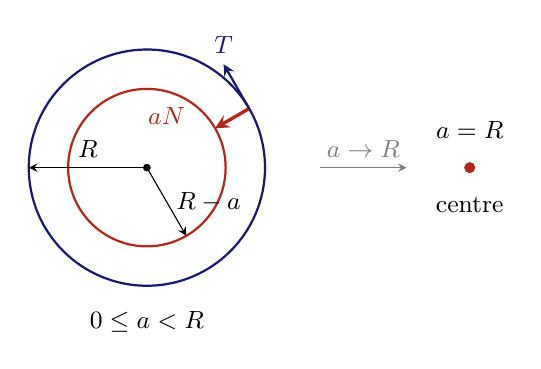
\begin{tikzpicture}[x=1cm,y=1cm,font=\small,>=stealth]
\draw[MidnightBlue,thick] (0,0) circle (1.5);
\draw[BrickRed,thick] (0,0) circle (1);
\fill (0,0) circle (1.4pt);
\draw[->] (0,0)--node[above] {$R$}(-1.5,0);
\draw[->] (0,0)--node[right] {$R-a$}(-60:1);
\draw[BrickRed,very thick,->] (30:1.5)--(30:1);
\node[BrickRed] at (.25,.65) {$aN$};
\draw[MidnightBlue,thick,->] (30:1.5)--++(120:.65) node[above] {$T$};
\node[below] at (0,-1.7) {$0\le a<R$};
\draw[gray,->] (2.2,0)--node[above] {$a\to R$}(3.3,0);
\fill[BrickRed] (4.1,0) circle (2pt);
\node[below] at (4.1,-.25) {centre};
\node[above] at (4.1,.25) {$a=R$};
\end{tikzpicture}
